\documentclass[paper=a4, fontsize=11pt]{scrartcl}
\usepackage[utf8]{inputenc} 
\usepackage[T1]{fontenc}
\usepackage{fourier}

\usepackage[english]{babel}
\usepackage[protrusion=true,expansion=true]{microtype}	
\usepackage{amsmath,amsfonts,amsthm} % Math packages
\usepackage[pdftex]{graphicx}
\usepackage[normalem]{ulem}
\usepackage{hyperref}

\usepackage[ruled]{algorithm2e} % For algorithms
\renewcommand{\algorithmcfname}{ALGORITHM}

%%% Custom sectioning
\usepackage{sectsty}
\allsectionsfont{\centering \normalfont\scshape}


%%% Custom headers/footers (fancyhdr package)
\usepackage{fancyhdr}
\pagestyle{fancyplain}
\fancyhead{}											% No page header
\fancyfoot[L]{}
\fancyfoot[C]{\thepage}
\fancyfoot[R]{}
\renewcommand{\headrulewidth}{0pt}
\renewcommand{\footrulewidth}{0pt}
\setlength{\headheight}{13.6pt}


%%% Equation and float numbering
\numberwithin{equation}{section}	 % Equationnumbering: section.eq#
\numberwithin{figure}{section}	 % Figurenumbering: section.fig#
\numberwithin{table}{section}	 % Tablenumbering: section.tab#


%%% Maketitle metadata
\newcommand{\horrule}[1]{\rule{\linewidth}{#1}} 	% Horizontal rule

\title{
		%\vspace{-1in} 	
		\usefont{OT1}{bch}{b}{n}
		\normalfont \normalsize \textsc{Case Western Reserve University} \\ [25pt]
		\horrule{0.5pt} \\[0.4cm]
		\huge Egyptian Fractions: Algorithms and Problems \\
		\horrule{2pt} \\[0.5cm]
}
\author{
		\normalfont 			\normalsize
        Mark Lalor\\[-3pt]		\normalsize
        Brian Li\\[-3pt]		\normalsize
        \\
        \today
}
\date{}


%%% Begin document
\begin{document}
\maketitle
\section{Introduction}
An Egyptian fraction is an expansion of a positive rational number as a sum of (usually distinct) unit fractions. Unit fractions are fractions with $1$ in the numerator and a positive integer in the denominator. That is, the representation of a rational number $p/q$ as:
\begin{equation}
	\frac{p}{q} = \frac{1}{a_1} + \frac{1}{a_2} + \ldots + \frac{1}{a_n}
\end{equation}
\subsection{History}
Usage of Egyptian fractions by Egyptians is evidenced by the Rhind Papyrus which is a document that dates back to 1550 BCE \cite{imhausen}. The Rhind Papyrus gets its name from Henry Rhind who purchased the document in 1858 \cite{imhausen}. In the Rhind Papyrus, there is a table of Egyptian Fraction representations for fractions of the form $\frac{2}{n}$ (where n is odd) and Egyptian fraction practice problems with corresponding solutions \cite{imhausen}. With the advent of computational theory, new problems involving Egyptian fractions have appeared such as the computation complexity of computing Egyptian Fraction of a fraction in the fewest terms possible and the Erd\H{o}s-Straus Conjecture [6].
\subsection{Properties}
Egyptian fractions can be used to solve questions concerning division of a quantity among multiple parties where the division may not be even. For example, consider the problem of dividing 5 loaves of bread among 7 people: $5/7 = 1/2 + 1/7 + 1/14$. Without the expansion, all 5 loaves would need to be divided into sevenths, then 5 of each seventh would go to each person. With the expansion, 4 loaves can be cut into halves, each person receiving a half piece. The remaining half loaf can be cut into sevenths (these would be fourteenths), and each person would receive a fourteenth. There remains one loaf of bread which we can cut into sevenths and evenly distribute among all 7 people. In total, we performed $4 + 6 + 6 = 16$ cuts. Without the expansion, we would need to perform $5 \times 6 = 30$ cuts.

Beyond the application of dividing quantities, several mathematicians found interesting properties associated with Egyptian fractions. For instance, Fibonacci was able to prove that any fraction could be represented as a finite sum of distinct unit fractions \cite{dunton}.

\section{Algorithms}
\subsection{Fibonacci's Greedy Algorithm}
\begin{algorithm}[t]
\KwIn{A fraction with numerator $x$ and denominator $y$ in lowest terms.}
\KwOut{A set $S$ of fractions with unit numerators such that $\sum\limits_{t \in S} t=\frac{x}{y}$}
\eIf{$x=1$}{
	\KwRet $\bigg\{\frac{1}{y}\bigg\}$
}{
	 $k \longleftarrow \bigg\lceil\frac{y}{x}\bigg\rceil$
	 
	 $\frac{x'}{y'} \longleftarrow \frac{x}{y} - \frac{1}{k}$ such that $\frac{x'}{y'}$ is in lowest terms.
	 
	 \KwRet $\bigg\{\frac{1}{k}\bigg\}\:\bigcup\:\textsc{fib-greedy}\left(\frac{x'}{y'}\right)$
	 
}

\caption{\textsc{fib-greedy}: Fibonacci's Greedy Algorithm}
\label{alg:one}
\end{algorithm}
Fibbonaci's greedy algorithm can be stated as follows: subtract out the largest possible unit fraction from the original fraction (that is, the largest fraction that does not result in a negative number after subtraction), then recurse on the result. The motivation of this algorithm is to decrease the remaining fractional value as fast as possible. The algorithm's implementation is demonstrated in more detail in Algorithm \ref{alg:one}. We explore some of the observed consequences of this greedy approach in Section \ref{sec:optimality}.

It simple to show by induction that the algorithm returns a valid expansion, however it is less clear whether the algorithm will always terminate. We present a proof that Fibonacci’s greedy algorithm always terminates:

Let us start with a rational number, $\frac{p}{q}$. In our greedy expansion, we have:
\begin{equation}\label{greedy1}
	\frac{p}{q} = \frac{1}{a_1} + \frac{1}{a_2} + \ldots + \frac{1}{a_n}
\end{equation}
Let us also add an ordering constraint:
\begin{equation}
	a_1 < a_2 < \ldots < a_n
\end{equation}

Now that we have the problem set up, our goal is to now show that equation \ref{greedy1} is a finite sequence. We will do this by showing that the first step forces the numerator of the following term to be smaller than the numerator of the original term. If we show that for the first step, then we can show that the numerators of the remainders of each step of the algorithm monotonically decrease until the numerator is equal to 1; in which case, we would have the final unitary fraction.

We will start by manipulating the remainder of subtracting $1/a_1$ from $p/q$:
\begin{equation}
	\frac{p}{q} - \frac{1}{a_1} = \frac{pa_1 - q}{qa_1}
\end{equation}

Next we will make use of the inequality:
\begin{equation}
	\frac{1}{a_1 - 1} > \frac{p}{q}
\end{equation}

This inequality comes from the fact that a1 is the smallest denominator such that $1/a_1 < p/q$ which means a unitary fraction with a smaller denominator than $a_1$ would be greater than $p/q$. With some algebraic manipulation, we find:

\begin{equation}\label{greedy2}
\begin{split}
	\frac{1}{a_1 - 1} > \frac{p}{q} \\
	q > p(a_1 - 1) \\
	q > pa_1 - p \\
	p > pa_1 - q \\
\end{split}
\end{equation}

From equation \ref{greedy2}, we can see that the numerator of the original term, $p$, is strictly larger than the numerator of the remainder term, $pa_1 - q$. Thus, we have shown that Fibonacci’s greedy algorithm terminates.

\subsection{Odd Greedy Algorithm}
In the odd greedy algorithm, the only difference is that it picks the largest unitary fraction but with the restriction that the denominator is odd. Unlike Fibonacci's greedy algorithm, it has remained unproven whether or not the greedy algorithm always terminates, no examples have shown that it does not. We discuss this open problem in more detail in Section \ref{sec:oddgreedy}. We demonstrate more precisely the implementation of this algorithm in Algorithm \ref{alg:two}.

\begin{algorithm}[t]
\KwIn{A fraction with numerator $x$ and denominator $y$ in lowest terms.}
\KwOut{A set $S$ of fractions with unit numerators and odd denominators such that $\sum\limits_{t \in S} t=\frac{x}{y}$}
\eIf{$x=1$}{
	\KwRet $\bigg\{\frac{1}{y}\bigg\}$
}{
	 $n \longleftarrow$ the smallest integer such that $n \geq \frac{y}{x}$ and $n \equiv 1 \pmod{2}$.
	 
	 $\frac{x'}{y'} \longleftarrow \frac{x}{y} - \frac{1}{n}$ such that $\frac{x'}{y'}$ is in lowest terms.
	 
	 \KwRet $\bigg\{\frac{1}{n}\bigg\}\:\bigcup\:\textsc{odd-greedy}\left(\frac{x'}{y'}\right)$
	 
}
\caption{\textsc{odd-greedy}: Odd Greedy Algorithm}
\label{alg:two}
\end{algorithm}

\subsection{Brute Force Shortest Algorithm}
In \cite{stewart}, Stewart tells a story about two men who come across the Diophantine equation:
\begin{equation}
	\frac{1}{a} + \frac{1}{b} + \frac{1}{c} + \frac{1}{d} = 1
\end{equation}
One of the men in the story, Mustapha, enumerated all the solutions to this Diophantine equation. To do so, Mustapha introduced the constraint:
\begin{equation}\label{brute1}
	a < b < c < d
\end{equation}

With this constraint, Mustapha could systematically try all potentially valid values for $a$,$b$,$c$, and $d$. For instance, to solve the above Diophantine equation, $a$ cannot be smaller than 4 because if $a=5$, any assignment of $b$,$c$, and $d$ with constraint \ref{brute1} will be less than 1. Though Mustapha used his brute force for four unit fractions, his approach can also be generalized to $n$ unit fractions:

\begin{equation}
	\frac{1}{a_1} + \frac{1}{a_2} + \ldots + \frac{1}{a_n} = 1
\end{equation}

\begin{equation}\label{brute2}
	a_1 < a_2 < \ldots < a_n
\end{equation}

In addition to generalizing Mustapha’s brute approach to a variable number of unit fractions, his approach can also be generalized for summing to any positive rational number:
\begin{equation}\label{brute_p}
	\frac{1}{a_1} + \frac{1}{a_2} + \ldots + \frac{1}{a_n} = p
\end{equation}

Equipped with the ability to use brute force for finding all solutions for equation \ref{brute_p}, we can find the shortest Egyptian Fraction for any positive rational number, $p$, by trying Mustapha’s brute force approach for 1, 2, … until we find a solution.

The solution returned by this algorithm will be the shortest Egyptian Fraction for the rational number p. We can prove this by assuming that there exists an "optimal" Egyptian Fraction, $O$, shorter than the expansion we returned from the algorithm, $E$. Since the generalization of Mustapha’s brute force approach would have enumerated and checked all expansions $< \|E\|$, our algorithm must have found $O$ and not returned it because it was not a valid Egyptian Fraction for $p$. Thus, we arrive at a contradiction that $O$ is not a valid Egyptian Fraction. 

\subsection{Optimality of the Greedy Algorithm}\label{sec:optimality}
It is interesting to see how the Egyptian fractions derived from Fibonacci’s greedy algorithm diverge from the "optimal" solutions generated by the brute-force approach. We evaluated the brute-force and greedy algorithms for fractions $\frac{x}{y}$ where $x,y \leq n$ for $n=500$ to investigate these differences (materials available at \href{https://github.com/marklalor/number-theory-report}{github.com/marklalor/number-theory-report}). Unsurprisingly, the frequency of matching results decreases as the fractions' components grow larger. However, for small $n$, it is notable that the greedy algorithm finds the optimal solution quite frequently as can be seen in Figure \ref{fig:n_freq}

\begin{figure}[t]
\centering
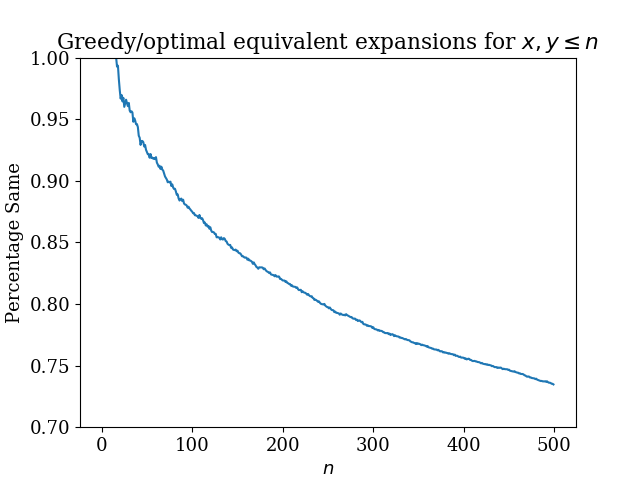
\includegraphics[width=0.60\textwidth]{n_percent_graph}
\caption{Frequency of optimal Egyptian fractions found by the greedy algorithm for all fractions of the form $\frac{x}{y}$ such that $x,y \leq n$.}
\label{fig:n_freq}
\end{figure}

In order to analyze some other patterns or interesting results of the solutions, we quantify the \textbf{disparity} between algorithm solutions in two ways:
\begin{enumerate}
	\item \textbf{term disparity}: the difference in number of terms between the greedy and optimal expansions.
	\item \textbf{denominator disparity}: the difference in the magnitudes of the largest denominators between the greedy and optimal expansions.
\end{enumerate}

We plot the term disparity between the greedy and optimal expansions with darker pixels for higher term disparity at point $(x,y)$ for fraction $\frac{x}{y}$ in Figure \ref{fig:term_disp}.

\begin{figure}[t]
\centering
\fbox{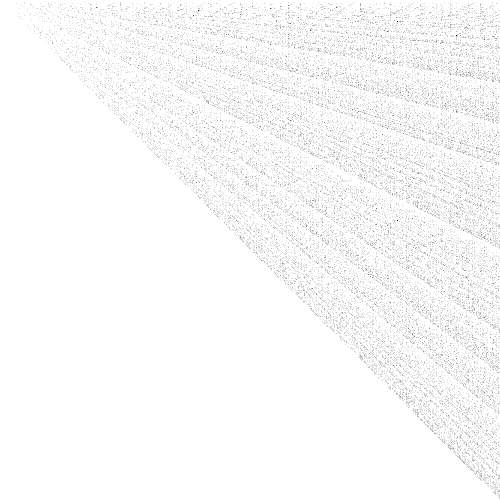
\includegraphics[width=0.75\textwidth]{pixel_terms}}
\caption{Term disparity between Fibonacci and optimal expansions for $\frac{x}{y}$. Higher term disparity is represented by darker pixels, while white represents zero term disparity.}
\label{fig:term_disp}
\end{figure}

An interesting feature of the term disparities in this sample is that the maximum disparity is much smaller in magnitude compared to the magnitudes of $x$ and $y$. While $x$ and $y$ can be up to $500$, the maximum term disparity is $8$. We find several fractions with term disparities of $8$, noted in Figure \ref{fig:disparity}.

There are clear patterns in the distribution of the optimal and unoptimal greedy expansions. We notice immediately in the middle of the image we have a line that lie near multiples of $1/2$. Lines that appear above this center one are near a multiple of $1/n$. Lines below the center are near multiples of $(n-1)/n$

We also take a look at some of expansions with worst denominator disparity in the sample set. We find that that expansions with the highest denominator disparities are also often the same as those with the highest term disparities, the largest being $\frac{36}{457}$ with denominator disparity of $2837$! These can also be seen in Figure \ref{fig:disparity} alongside term disparity.

\begin{figure}[t]
\centering
\begin{tabular}{|c|c|c|c|}
    \hline
    \multicolumn{2}{|c|}{\textbf{fraction}} & \multicolumn{2}{|c|}{\textbf{disparity}} \\ \hline
	\textbf{x} & \textbf{y} & \textbf{term} & \textbf{denominator} \\ \hline\hline
	36 & 457 & 8 & 2837 \\ \hline
	11 & 199 & 8 & 1343 \\ \hline
    22 & 398 & 8 & 1343 \\ \hline
    221 & 398 & 8 & 1343 \\ \hline
    9 & 271 & 6 & 390 \\ \hline
    31 & 311 & 6 & 529 \\ \hline
\end{tabular}
\caption{High term and denominator disparities (base 10) for exemplary fractions.}
\label{fig:disparity}
\end{figure}
 
\section{Open Problems}
\subsection{Efficient Shortest Egyptian Fraction}

In our algorithms section we showed that a brute force approach exists for finding the shortest Egyptian fraction (in number of terms in the expansion) for a rational number, $p$ such that $0 < p < 1$. However, there are two interesting questions to continue investigating: What is the runtime complexity of our algorithm and does there exist a more efficient solution for this problem? Depending on the answer to the latter question, we might also ask: Is the problem of finding the shortest Egyptian fraction NP-complete or NP-hard?

First, we will take a look at runtime complexity of our algorithm. For runtime complexity, we want to express the runtime of our algorithm in terms of our input size. If we consider a rational number, $p$ with a numerator $N$, Fibonacci’s greedy algorithm guarantees us an Egyptian Fraction of length $l \leq N$ \cite{graham}. Now that we have an upper-bound on the size of our Egyptian Fraction, we can see that our algorithm will take $O(x^N)$ where $x$ is the max number of possibilities that any $a_i$ can take on in equation \ref{brute_p}. There may exist a tighter upper-bound, but with this analysis, it seems like our brute force approach is exponential in runtime.

Next, we will take a look at the next few questions on an optimal algorithm. Based on the existing literature, it seems like the tractability of finding the shortest Egyptian fraction is an open problem. One method to prove that the problem is tractable is to find an algorithm that finds the shortest expansions in polynomial time. If the problem is in fact not tractable, then we can prove it by showing that an existing NP-complete problem (e.g. \textsc{SAT}, \textsc{VERTEX-COVER}, etc.) can be reduced to the Egyptian fraction problem. In other words, if we can solve a known NP-complete problem by solving a specific instance of the Egyptian fraction problem, then we have shown that finding the shortest expansion is at least as hard as an intractable problem.

\subsection{Erd\H{o}s–Straus Conjecture}
The Erd\H{o}s–Straus Conjecture may be stated as follows:
For every $n \geq 2$, there exists integers $x$, $y$, $z$ such that:

\begin{equation}\label{erdos}
	\frac{4}{n} = \frac{1}{x} + \frac{1}{y} + \frac{1}{z}
\end{equation}

With brute-force computer aid, the conjecture has been proved for $n \leq 1017$. However, there does not currently exist a proof for all $n$.

Work has been done to show the form that counterexamples would take on. Of particular interest is the form of the smallest $n$ that is a counterexample. If the smallest counterexample was a composite number, then the solution for the composing primes could be found first, therefore it is a contradiction that the smallest $n$ is composite and therefore it is prime.

Additionally, Mordell proved that if a solution is prime, it is congruent to one of $12$, $112$, $132$, $172$, $192$, or $232 \pmod{840}$\:\cite{mordell}, therefore the smallest counterexample $n$ would also be a member of one of these sequences.
\subsection{Correctness of the Odd Greedy Algorithm}\label{sec:oddgreedy}
In \cite{starke}, Starke et. al show that a finite odd Egyptian fraction exists for all positive rational numbers with odd denominators. However, they do not show whether an \textit{odd greedy expansion} exists for all positive rational numbers with odd denominators. An odd greedy expansion is a special case of the Egyptian fraction which is generated by the odd greedy algorithm. In \cite{guy}, Stein, Selfridge, Graham are given credit for posing the question: “If $m/n$, a rational number ($n$ odd), is expressed as $\sum \frac{1}{x_i}$, where the $x_i$ are successively chosen to be the least possible odd integers which leave a nonnegative remainder, is the sum always finite?” So far, Kertesz has checked this conjecture for $2 < m < n < 120$ \cite{guy}. However, for some rational numbers, the odd greedy expansion can yield unitary fractions with pathologically large denominators. For example, David Bailey found that $5/5809$ yielded a unitary fraction with over $60,000,000$ decimal digits \cite{guy}. Currently, it is unknown whether all rational numbers with odd denominators have an odd greedy expansion, since it has not yet been proven that the odd greedy algorithm always terminates or that a counterexample for the conjecture exists.


\begin{thebibliography}{9}
	\bibitem{nazario}
	Arce-Nazario, R., F. Castro, and R. Figueroa.
	\textit{On the Number of Solutions of} \:\:$\sum_{i=1}^{11} \frac{1}{x_i} = 1$ \textit{in Distinct Odd Natural Numbers.}
	Journal of Number Theory, vol. 133, no. 6, 2013, pp. 2036-2046.
	\bibitem{mordell}
	Mordell, Louis J.
	\textit{Diophantine Equations}.
	vol. 30, Academic Press, New York, 1969. pp. 287–288
	\bibitem{elsholtz}
	Elsholtz, Christian.
	\textit{Egyptian Fractions with Odd Denominators}.
	Quarterly Journal of Mathematics, vol. 67, no. 3, 2016, pp. 425-430.
	\bibitem{pihko}
	Pihko, J.
	\textit{Remarks on the "Greedy Odd" Egyptian Fraction Algorithm Ii.}
	Fibonacci Quarterly, vol. 48, no. 3, 2010, pp. 202-208.
	\bibitem{stewart}
	I. Stewart,
	\textit{The Riddle of the Vanishing Camel},
	Scientific American, vol. 266, no. 6, pp. 122–124, 1992.
	\bibitem{dunton}
	Dunton, M.
	\textit{Fibonacci on Egyptian Fractions},
	Fibonacci Quarterly, vol. 4, no. 4, 1966, pp. 339-354
	\bibitem{graham}
	R. L. Graham,
	\textit{Paul Erd\H{o}s and Egyptian Fractions},
	Bolyai Society Mathematical Studies Erd\H{o}s Centennial, pp. 289–309, 2013.
	\bibitem{starke}
	E. P. Starke and R. Breusch,
	\textit{4512},
	The American Mathematical Monthly, vol. 61, no. 3, p. 200, 1954.
	\bibitem{guy}
	Guy, Richard,
	\textit{Unsolved Problems in Number Theory},
	pp. 252-259,
	1981.
	\bibitem{imhausen}
	Imhausen, Annette,
	\textit{Mathematics in Ancient Egypt: A Contextual History},
	pp. 65-67,
	2016.
	
\end{thebibliography}

%\bibliographystyle{mla}
%\bibliography{bibliography}

%%% End document
\end{document}